% -*- compile-command: "pdflatex mikro.tex"; eval: (compile-on-save-mode) -*-

\documentclass[a4paper,12pt]{article}
\usepackage[utf8]{inputenc}
\usepackage[swedish]{babel}
\usepackage[margin=2cm]{geometry}
\usepackage{graphicx}
\usepackage{fix-cm}


\usepackage{tgadventor}
\renewcommand*\familydefault{\sfdefault}
\usepackage[T1]{fontenc}

\pagestyle{empty}


\begin{document}
\linespread{2}
\centering

\begin{figure}
  \centering
  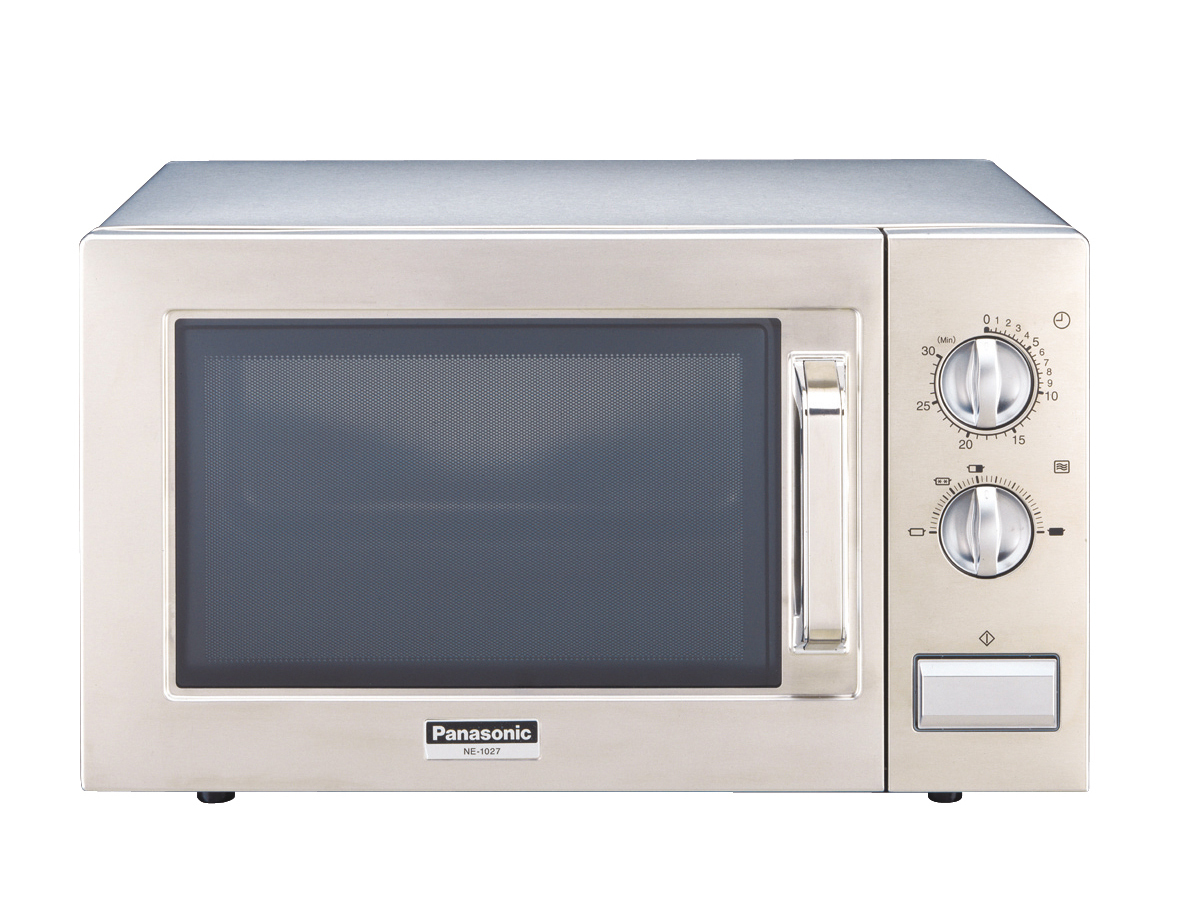
\includegraphics[width=0.8\textwidth]{mikro.jpg}
\end{figure}

\mbox{}
\vspace{0.1cm}


\fontsize{30}{20}\selectfont\normalfont
Välkommen Nollan!\\
Här på CYD-poolen har vi

\fontsize{60}{40}\selectfont\normalfont
Resturang\-mikrovågsugnar\\

\vspace{0.8cm}
\fontsize{30}{20}\selectfont\normalfont
som värmer yttepyttelite bättre än ugnarna i universitetets alla dåliga kök. Så tänk på det nollan.


\end{document}
